% !TeX root = ../main.tex
% Add the above to each chapter to make compiling the PDF easier in some editors.

\section{Novelty and Diversity}\label{section:novelty_and_diversity}

\subsection{Introduction}
[kopi peyst. handbook chapter 26]
Accurately predicting the users’ interests was the main direct or implicit drive of the recommender systems field in roughly the first decade and a half of the field’s development. A wider perspective towards recommendation utility, including but beyond prediction accuracy, started to appear in the literature by the beginning of the 2000s [36, 70], taking views that began to realize the importance of novelty and diversity, among other properties, in the added value of recommendation [53, 90]. This realization grew progressively, reaching an upswing of activity by the turn of the past decade [1, 3, 20, 39, 75]. Today we might say that novelty and diversity are becoming an increasingly frequent part of evaluation practice. They are being included increasingly often among the reported effectiveness metrics of new recommendation approaches, and are explicitly targeted by algorithmic innovations time and again. And it seems difficult to conceive progress in the recommender systems field without considering these dimensions and further developing our understanding thereof. Even though dealing with novelty and diversity remains an active area of research and development, considerable progress has been achieved in these years in terms of the development of enhancement techniques, evaluation metrics, methodologies, and theory, and we deem the area is therefore ripe for a broad overview as we undertake in this chapter.

In this chapter we analyze the different motivations, notions and perspectives under which novelty and diversity can be understood and defined (Sect.26.2). We revise the evaluation procedures and metrics which have been developed in this area (Sect. 26.3), as well as the algorithms and solutions to enhance novelty and/or diversity (Sect. 26.4). We analyze the relationship with the recent and prolific stream of work on diversity in Information Retrieval, as a confluent area with recommender systems, and discuss a unifying framework that aims to provide a common basis as comprehensive as possible to explain and interrelate different novelty and diversity perspectives (Sect. 26.5). We show some empirical results that illustrate the behavior of metrics and algorithms (Sect. 26.6), and close the chapter with a summary and discussion of the progress and perspectives in this area, and directions for future research (Sect. 26.7).

\subsection{Novelty and Diversity in Recommender Systems}

Novelty can be generally understood as the difference between present and past experience, whereas diversity relates to the internal differences within parts of an experience. The difference between the two concepts is subtle and close connections can in fact be established, depending on the point of view one may take, as we shall discuss. The general notions of novelty and diversity can be particularized in different ways. For instance, if a music streaming service recommends us a song we have never heard before, we would say this recommendation brings some novelty. Yet if the song is, say, a very canonical music type by some very well known singer, the involved novelty is considerably less than we would get if the author and style of the music were also original for us. We might also consider that the song is even more novel if, for instance, few of our friends know about it. On the other hand, a music recommendation is diverse if it includes songs of different styles rather than different songs of very similar styles, regardless of whether the songs are original or not for us. Novelty and diversity are thus to some extent complementary dimensions, though we shall seek and discuss in this chapter the relationships between them.
The motivations for enhancing the novelty and diversity of recommendations are manifold, as are the different angles one may take when seeking these qualities. This is also the case in other fields outside information systems, where novelty and diversity are recurrent topics as well, and considerable efforts have been devoted to casting clear definitions, equivalences and distinctions. We therefore start this chapter by overviewing the reasons for and the possible meanings of novelty and diversity in recommender systems, with a brief glance at related perspectives in other disciplines.

\subsubsection{Why Novelty and Diversity in Recommendation}

Bringing novelty and diversity into play as target properties of the desired outcome means taking a wider perspective on the recommendation problem concerned with final actual recommendation utility, rather than a single quality side such as accuracy [53]. Novelty and diversity are not the only dimensions of recommendation utility one should consider aside from accuracy (see e.g. Chap. 8 for a comprehen- sive survey), but they are fundamental ones. The motivations for enhancing novelty and diversity in recommendations are themselves diverse, and can be founded in the system, user and business perspectives.

From the system point of view, user actions as implicit evidence of user needs involve a great extent of uncertainty as to what the actual user preferences really are. User clicks and purchases are certainly driven by user interests, but identifying what exactly in an item attracted the user, and generalizing to other items, involves considerable ambiguity. On top of that, system observations are a very limited sample of user activity, whereby recommendation algorithms operate on significantly incomplete knowledge. Furthermore, user interests are complex, highly dynamic, context-dependent, heterogeneous and even contradictory. Predicting the user needs is therefore an inherently difficult task, unavoidably subject to a non- negligible error rate. Diversity can be a good strategy to cope with this uncertainty and optimize the chances that at least some item pleases the user, by widening the range of possible item types and characteristics at which recommendations aim, rather than bet for a too narrow and risky interpretation of user actions. For instance, a user who has rated the movie “Rango” with the highest value may like it because— in addition to more specific virtues—it is a cartoon, a western, or because it is a comedy. Given the uncertainty about which of the three characteristics may account for the user preference, recommending a movie of each genre generally pays off more than recommending, say three cartoons, as far as three hits do not necessarily bring three times the gain of one hit—e.g. the user might rent just one recommended movie anyway—whereas the loss involved in zero hits is considerably worse than achieving a single hit. From this viewpoint we might say that diversity is not necessarily an opposing goal to accuracy, but in fact a strategy to optimize the gain drawn from accuracy in matching true user needs in an uncertain environment.

On the other hand, from the user perspective, novelty and diversity are generally desirable per se, as a direct source of user satisfaction. Consumer behaviorists have long studied the natural variety-seeking drive in human behavior [51]. The explanation of this drive is commonly divided into direct and derived motivations. The former refer to the inherent satisfaction obtained from “novelty, unexpect- edness, change and complexity” [50], and a genuine “desire for the unfamiliar, for alternation among the familiar, and for information” [64], linking to the existence of an ideal level of stimulation, dependent on the individual. Satiation and decreased satisfaction results from the repeated consumption of a product or product characteristic in a decreasing marginal value pattern [25]. As preferences towards discovered products are developed, consumer behavior converges towards a balance between alternating choices and favoring preferred products [16]. Derived motivations include the existence of multiple needs in people, multiple situations, or changes in people’s tastes [51]. Some authors also explain diversity-seeking as a strategy to cope with the uncertainty about one’s own future preference when one will actually consume the choices [44], as e.g. when we choose books and music for a trip. Moreover, novel and diverse recommendations enrich the user experience over time, helping expand the user’s horizon. It is in fact often the case that we approach a recommender system with the explicit intent of discovering something new, developing new interests, and learning. The potential problems of the lack of diversity which may result from too much personalization has recently come to the spotlight with the well-known debate on the so-called filter bubble [60]. This controversy adds to the motivation for reconciling personalization with a healthy degree of diversity.

Diversity and novelty also find motivation in the underlying businesses in which recommendation technologies are deployed. Customer satisfaction indirectly benefits the business in the form of increased activity, revenues, and customer loyalty. Beyond this, product diversification is a well-known strategy to mitigate risk and expand businesses [49]. Moreover, selling in the long tail is a strategy to draw profit from market niches by selling less of more and getting higher profit margins on cheaper products [9].

All the above general considerations can be of course superseded by particular characteristics of the specific domain, the situation, and the goal of the recommen- dations, for some of which novelty and diversity are indeed not always needed. For instance, getting a list of similar products (e.g. photo cameras) to one we are currently inspecting may help us refine our choice among a large set of very similar options. Recommendations can serve as a navigational aid in this type of situation. In other domains, it makes sense to consume the same or very similar items again and again, such as grocery shopping, clothes, etc. The added value of recommendation is probably more limited in such scenarios though, where other kinds of tools may solve our needs (catalog browsers, shopping list assistants, search engines, etc.), and even in these cases we may appreciate some degree of variation in the mix every now and then.

\subsubsection{Defining Novelty and Diversity}

Novelty and diversity are different though related notions, and one finds a rich variety of angles and perspectives on these concepts in the recommender system literature, as well as other fields such as sociology, economy, or ecology. As pointed out at the beginning of this section, novelty generally refers, broadly, to the difference between present and past experience, whereas diversity relates to the internal differences within parts of an experience. Diversity generally applies to a set of items or “pieces”, and has to do with how different the items or pieces are with respect to each other. Variants have been defined by considering different pieces and sets of items. In the basic case, diversity is assessed in the set of items recommended to each user separately (and typically averaged over all users afterwards) [90]. But global diversity across sets of sets of items has also been considered, such as the recommendations delivered to all users [3, 4, 89], recommendations by different systems to the same user [11], or recommendations to a user by the same system over time [46].

The novelty of a set of items can be generally defined as a set function (average, minimum, maximum) on the novelty of the items it contains. We may therefore consider novelty as primarily a property of individual items. The novelty of a piece of information generally refers to how different it is with respect to “what has been previously seen” or experienced. This is related to novelty in that when a set is diverse, each item is “novel” with respect to the rest of the set. Moreover, a system that promotes novel results tends to generate global diversity over time in the user experience; and also enhances the global “diversity of sales” from the system perspective. Multiple variants of novelty arise by considering the fact that novelty is relative to a context of experience, as we shall discuss.

Different nuances have been considered in the concept of novelty. A simple definition of novelty can consist of the (binary) absence of an item in the context of reference (prior experience). We may use adjectives such as unknown or unseen for this notion of identity-based novelty [75]. Long tail notions of novelty are elaborations of this concept, as they are defined in terms of the number of users who would specifically know an item [20, 61, 89]. But we may also consider how different or similar an unseen item is with respect to known items, generally— but not necessarily—on a graded scale. Adjectives such as unexpected, surprising and unfamiliar have been used to refer to this variant of novelty. Unfamiliarity and identitary novelty can be related by trivially defining similarity as equality, i.e. two items are “similar” if and only if they are the same item. Finally, the notion of serendipity is used to mean novelty plus a positive emotional response— in other words, an item is serendipitous if it is novel—unknown or unfamiliar—and relevant [57, 88].

The present chapter is concerned with the diversity and novelty involved in recommendations, but one might also study the diversity (in tastes, behavior, demographics, etc.) of the end-user population, or the product stock, the sellers, or in general the environment in which recommenders operate. While some works in the field have addressed the diversity in user behavior [31, 72], we will mostly focus on those aspects a recommender system has a direct hold on, namely the properties of its own output.

\subsubsection{Diversity in Other Fields}

Diversity is a recurrent theme in several fields, such as sociology, psychology, economy, ecology, genetics or telecommunications. One can establish connections and analogies from some—though not all—of them to recommender systems, and some equivalences in certain metrics, as we will discuss.

Diversity is a common keyword in sociology referring to cultural, ethnic or demographic diversity [47]. Analogies to recommender system settings would apply to the user population, which is mainly a given to the system, and therefore not within our main focus here. In economy, diversity is extensively studied in relation to different issues such as the players in a market (diversity vs. oligopolies), the number of different industries in which a firm operates, the variety of products commercialized by a firm, or investment diversity as a means to mitigate the risk involved in the volatility of investment value [49]. Of all such concepts, product and portfolio diversity most closely relate to recommendation, as mentioned in Sect. 26.2.1, as a general risk-mitigating principle and/or business growth strategy.

Behaviorist psychology has also paid extensive attention to the human drive for novelty and diversity [51]. Such studies, especially the ones focusing on consumer behavior, provide formal support to the intuition that recommender system users may prefer to find some degree of variety and surprise in the recommendations they receive, as discussed in Sect. 26.2.1.

An extensive strand or literature is devoted to diversity in ecology as well, where researchers have worked to considerable depth on formalizing the problem, defining and comparing a wide array of diversity metrics, such as the number of species (richness), Gini-Simpson and related indices, or entropy [62]. Such developments connect to aggregate recommendation diversity perspectives that deal with sets of recommendations as a whole, as we shall discuss in Sects. 26.2.3 and 26.5.3.3.

Finally, the issue of diversity has also attracted a great deal of attention in the Information Retrieval (IR) field. A solid body of theory, metrics, evaluation methodologies and algorithms has been developed in this scope in the last decade [6, 17, 21, 22, 24, 67, 84], including a dedicated search diversity task in four consecutive TREC editions starting in 2009 [23]. Search and recommendation are different problems, but have much in common: both tasks are about ranking a set of items to maximize the satisfaction of a user need, which may or may not have been expressed explicitly. It has in fact been found that the diversity theories and techniques in IR and recommender systems can be connected [77, 78], as we will discuss in Sect. 26.5.4. Given these connections, and the significant developments on diversity in IR, we find it relevant to include an overview of this work here, as we will do in Sects. 26.3 (metrics) and 26.4 (algorithms).

\subsection{Novelty and Diversity Evaluation}

The definitions discussed in the previous sections can only get a full, precise and practical meaning when one has given a specific definition of the metrics and methodologies by which novelty and diversity are to be measured and evaluated. We review next the approaches and metrics that have been developed to assess novelty and diversity, after which we will turn to the methods and algorithms proposed in the field to enhance them.

\subsubsection{Notation}

As is common in the literature, we will use the symbols i and j to denote items, u and v for users, I and U for the set of all items and users respectively. By $I_u$ and $U_i$ we shall denote, respectively, the set of all items u has interacted with, and the set of users who have interacted with i. In general we shall take the case where the interaction consists of rating assignment (i.e. at most one time per user-item pair), except where the distinction between single and multiple interaction makes a relevant difference (namely Sect. 26.5.2.1. We denote ratings assigned by users to items as $r ( u , i )$, and use the notation $r ( u , i ) = \emptyset$ to indicate missing ratings, as in [5]. We shall use R to denote a recommendation to some user, and $R_u$ whenever we wish or need to explicitly indicate the target user u to whom R is delivered— in other words, R will be a shorthand for $R_u$. By default, the definition of a metric will be given on a single recommendation for a specific target user. For notational simplicity, we omit as understood that the metric should be averaged over all users. Certain global metrics (such as aggregate diversity, defined in Sect. 26.3.5) are the exception to this rule: they directly take in the recommendations to all users in their definition, and they therefore do not require averaging. In some cases where a metric is the average of a certain named function (e.g. IUF for inverse user frequency, SI for self-information) on the items it contains, we will compose the name of the metric by prepending an “M” for “mean” (e.g. MIUF, MSI) in order to distinguish it from the item-level function.

\subsubsection{Average Intra-List Distance}

Perhaps the most frequently considered diversity metric and the first to be proposed in the area is the so-called average intra-list distance—or just intra-list diversity, ILD (e.g. [70, 85, 90]). The intra-list diversity of a set of recommended items is defined as the average pairwise distance of the items in the set:

$$\mathrm { ILD } = \frac { 1 } { | R | ( | R | - 1 ) } \sum _ { i \in R } \sum _ { j \in R } d ( i , j )$$


The computation of ILD requires defining a distance measure d(i, j), which is thus a configurable element of the metric. Given the profuse work on the development of similarity functions in the recommender systems field, it is common, handy and sensible to define the distance as the complement of well-understood similarity measures, but nothing prevents the consideration of other particular options. The distance between items is generally a function of item features [90], though the distance in terms of interaction patterns by users has also been considered sometimes [79].


The ILD scheme in the context of recommendation was first suggested, as far as we are aware of, by Smyth and McClave [70], and has been used in numerous subsequent works (e.g. [75, 79, 85, 90]). Some authors have defined this dimension by its equivalent complement intra-list similarity ILS [90], which has the same relation to ILD as the distance function has to similarity, e.g. ILD = 1 - ILS if d = 1- sim.

\subsubsection{Global Long-Tail Novelty}
[26.3.3]

\subsubsection{User-Specific Unexpectedness}
[26.3.4]

\subsubsection{Inter-Recommendation Diversity Metrics}
[26.3.5]

\subsubsection{Specific Methodologies}

As an alternative to the definition of special-purpose metrics, some authors have evaluated the novelty or diversity of recommendations by accuracy metrics on a diversity-oriented experimental design. For instance, Hurley and Zhang [39] evaluate the diversity of a system by its ability to produce accurate recommendations of difficult items, “difficult” meaning unusual or infrequent for a user’s typical observed habits. Specifically, a data splitting procedure is set up by which the test ratings are selected among a ratio of the top most different items rated by each user, “different” being measured as the average distance of the item to all other items in the user profile. The precision of recommendations in such a setting thus reflects the ability of the system to produce good recommendations made up of novel items. A similar idea is to select the test ratings among cold, non-popular long tail items. For instance, Zhou et al. [89] evaluate accuracy on the set of items with less than a given number of ratings. Shani and Gunawardana also discuss this idea in Chap. 8.

\subsubsection{Diversity vs. Novelty vs. Serendipity}
[26.3.7]

\subsection{Novelty and Diversity Enhancement Approaches}

Methods to enhance the novelty and diversity of recommendations are reviewed in this section. It is noteworthy that research in this area has accelerated over the last number of years. The work can be categorized into methods that re-rank an initial list to enhance the diversity/novelty of the top items; methods based on clustering; hybrid or fusion methods; and methods that consider diversity in the context of optimization of learning to rank objectives.

\subsubsection{Result Diversification/Re-ranking}
[26.4.1, onemli]

\subsubsection{Using Clustering for Diversification}

A method proposed in [86] clusters the items in an active user’s profile, in order to group similar items together. Then, rather than recommend a set of items that are similar to the entire user profile, each cluster is treated separately and a set of items most similar to the items in each cluster is retrieved.

A different approach is presented in [14], where the candidate set is again clustered. The goal now is to identify and recommend a set of representative items, one for each cluster, so that the average distance of each item to its representative is minimized.

A nearest-neighbor algorithm is proposed in [48] that uses multi-dimensional clustering to cluster items in an attribute space and select clusters of items as candidates to recommend to the active user. This method is shown to improve aggregate diversity.

A graph-based recommendation approach is described in [69] where the recom- mendation problem is formulated as a cost flow problem over a graph whose nodes are the users and items of the recommendation. Weights in the graph are computed by a biclustering of the user-item matrix using non-negative matrix factorization. This method can be tuned to increase the diversity of the resulting set, or increase the probability of recommending long-tail items.

\subsubsection{Fusion-Based Methods}

Since the early days of recommender systems, researchers have been aware that no single recommendation algorithm will work best in all scenarios. Hybrid systems have been studied to offset the strengths of one algorithm against the weaknesses of another (see [68] for example). It may be expected that the combined outputs of multiple recommendation algorithms that have different selection mechanisms, may also exhibit greater diversity than a single algorithm. For example, in [66, 79], recommendation is treated as a multi-objective optimization problem. The outputs of multiple recommendation algorithms that differ in their levels of accuracy, diversity and novelty are ensemble using evolutionary algorithms. As another example, in a music recommendation system called Auralist [88], a basic item- based recommender system is combined with two additional algorithms, in order to promote serendipity (see section below).

\subsubsection{Learning to Rank with Diversity}

In the last few years, there is an increasing interest in learning to rank algorithms for recommender systems. These algorithms directly optimize an objective related to the ranking rather than forming the ranking in a post-processing step from a set of predicted ratings. To date, most such techniques do not take into account the dependencies between the items in the ranking. However, a small number of works have appeared in the literature that optimize a combined objective of ranking accuracy and set diversity. In [71], the concept of diversity is integrated into a matrix factorization model, in order to directly recommend item sets that are both relevant and diversified. A matrix factorization model is again used in [40] to optimize a ranking objective that is explicitly modified to account for the diversity of the ranking.

\subsubsection{Other Approaches}

A nearest neighbor algorithm called usage-context based collaborative filtering (UCBCF) is presented in [58], which differs from standard item-based CF in the calculation of item-item similarities. Rather than the standard item representation as a vector of user ratings, an item profile is represented as a vector of the k other items with which the item significantly co-occurs in user profiles. UCBCF is shown to obtain greater aggregate diversity than standard kNN and Matrix Factorization algorithms. A system described in [8] maps items into a utility space and maps a user’s preferences to a preferred utility vector. In order to make a diverse recommendation, the utility space is split into m layers in increasing distance from the preferred utility and non-dominated items are chosen from each layer so as to maximize one dimension of the utility vector.

The works discussed so far have considered diversity in terms of the dissimilarity of items in a single recommendation set, or, in the case of aggregate diversity, the coverage of items in a batch of recommendations. Another approach is to consider diversity in the context of the behavior of the system over time. Temporal diversity (Eq.(26.7) in Sect.26.3.4) is investigated by Lathia et al. [46] in a number of standard CF algorithms, and methods for increasing diversity through re-ranking or hybrid fusion are discussed. In a related vein, Mourao et al. [56] explore the “oblivion problem”, that is, the possibility that in a dynamic system, items can be forgotten over time in such a way that they recover some degree of the original novelty value they had when they were discovered.

\subsubsection{User Studies}

It is one thing to develop algorithms to diversify top k lists, but what impact do these algorithms have on user satisfaction? A number of user studies have explored the impact of diversification on users. Topic diversification is evaluated in [90] by carrying out a user survey to assess user satisfaction with a diversified recommendation. In the case of their item-based algorithm, they find that satisfaction peaks around a relevance/diversity determined by $\lambda = 0.6$ in Eq. (26.9) suggesting that users like a certain degree of diversification in their lists.

While much of the work in diversifying top k lists does not consider the ordering of items in the recommended list, provided an overall relevance is attained, Ge et al. [32, 33] look at how this ordering affects the user’s perception of diversity. In a user study, they experiment with placing diverse items—ones with low similarity to the other items in the list—either in a block or dispersed throughout the list and found that blocking the items in the middle of the list reduces perceived diversity.

The work of Hu and Pu [37] addresses user-interface issues related to augmenting users’ perception of diversity. In a user study that tracks eye movements, they find that an organizational interface where items are grouped into categories is better than a list interface in supporting perception of diversity. In [19], 250 users are surveyed and presented with 5 recommendation approaches, with varying degrees of diversity. They find that users perceive diversity and that it improves their satisfaction but that diverse recommendations may require additional explanations to users who cannot link them back to their preferences.

\subsubsection{Diversification Approaches in Information Retrieval}

[26.4.8, eger kullanirsan]

\subsection{Unified View}

As the overview through this chapter shows, a wide variety of metrics and perspectives have been developed around the same concepts under different variants and angles. It is natural to wonder whether it is possible to relate them together under a common ground or theory, establishing equivalences, and identifying fundamental differences. We summarize next a formal foundation for defining, explaining, relating and generalizing many different state of the art metrics, and defining new ones. We also examine the connections between diversity as researched and developed in the Information Retrieval field, and the corresponding work in recommender systems.
[26.5, information retrieval'daki diverisity yi recommendation diversity'y bagliyor, kullanirsan kullan]

\subsection{Empirical Metric Comparison}
[26.6, Kendileri deney yapmislar ve sonuclari metriclere gore karsilastirmislar, kullanilabilir en azindan tablo]

\subsection{Conclusion}

The consensus is clear in the community on the importance of novelty and diversity as fundamental qualities of recommendations, and it seems difficult to make progress in the field without considering these dimensions. Considerable progress has been achieved in the area in defining novelty and diversity from several points of view, devising methodologies and metrics to evaluate them, and developing different methods to enhance them. This chapter aims to provide a wide overview on the work so far, as well as a unifying perspective linking them together as developments from a few basic common root principles.

It is our perception that work in this area is far from being finished. There is still room for further understanding the role of novelty and diversity, as well as theoretical, methodological and algorithmic developments around them. For instance, modeling feature-based novelty in probabilistic terms in order to unify discovery and familiarity models would be an interesting line for future work.

Aspects such as the time dimension, along which items may recover part of their novelty value [43, 56], or the variability among users regarding their degree of novelty-seeking trend, are examples of issues that require further research. Last but not least, user studies would bring considerable light as to whether the described metrics match the actual user perception, as well as the precise extent and conditions in which users appreciate novelty and diversity versus accuracy and other potential dimensions of recommendation effectiveness.

 \begin{figure}[!ht]
	\centering
	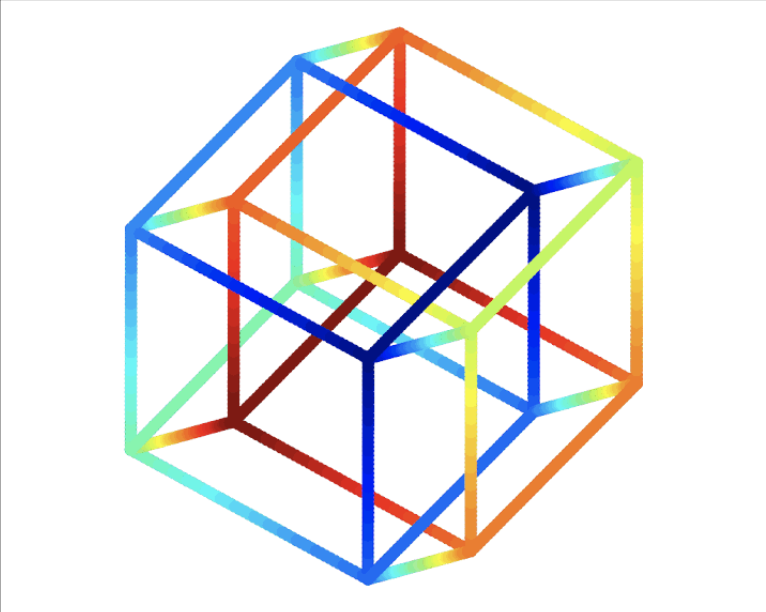
\includegraphics[width=0.75\textwidth]{figures/DimensionalityReduction.png}
	\caption{2D representation of a 4D cube. The colors indicate the depth in fourth dimension ~\parencite{lee2007nonlinear}.}
	\label{fig:embedding-projection-example}
\end{figure}

[TODO: burke2002hybrid -> tablolar]

